\documentclass[conference]{IEEEtran}
\IEEEoverridecommandlockouts
\usepackage{cite}
\usepackage{amsmath,amssymb,amsfonts}
\usepackage{graphicx}
\usepackage{textcomp}
\usepackage{xcolor}
\usepackage{booktabs}
\usepackage{url}
\usepackage{flushend}

\begin{document}

\title{NeuroShard: Useful-Work Mining for Decentralized Language Model Training\thanks{Prototype, experiment harnesses, and raw results: \protect\url{https://github.com/neuroshard-ai/neuroshard}. This work is unrelated to similarly named embedding-table and database-sharding systems.}}

\author{\IEEEauthorblockN{Linir Zamir}
\IEEEauthorblockA{\textit{Independent Researcher}\\
Boca Raton, FL, USA\\
lzamir2016@fau.edu}}

\maketitle

\begin{abstract}
NeuroShard aims to turn openly contributed computation into a shared language model and native token rewards. We propose useful-work mining: participants execute prescribed learning tasks, and NeuroShard's own blockchain settles verified contributions into model updates and token issuance. Tasks bind checkpoints, objectives, data, numerical semantics, and state transitions. Native consensus orders payments; neural verification checks the claimed work. A composition obstacle is that a minority of malicious pipeline stages can contaminate a majority of complete contributions. The design therefore requires dependency verification, availability, and resource-based admission. Component experiments show a 3.4\% validation-loss increase at $50\times$ lower outbound update payload; compression reaches $527\times$ with a 16.2\% increase. A separate native-chain demonstrator connects two model-stage workers to four validators using full replay and atomic rewards. Fifteen accepted steps reduce a fixed held-out batch loss from 5.74 to 4.11 and issue exactly 15 development tokens; outage and invalid-claim checks pass. These small-scale results establish an executable reference for auditable training settlement, while public admission, scalable verification, and economic sustainability remain open.
\end{abstract}

\begin{IEEEkeywords}
Decentralized machine learning, permissionless networks, verifiable computation, Byzantine fault tolerance, distributed training
\end{IEEEkeywords}

\section{Introduction}

Low-communication optimization and pipeline parallelism make geographically distributed language model training increasingly practical~\cite{douillard2023diloco,jaghouar2024opendiloco,jaghouar2024intellect,ryabinin2023swarm}. Permissionless participation adds different requirements: a public key does not identify an independent worker, a signed update does not prove correct computation, and agreement on a checkpoint does not imply learning quality.

NeuroShard targets a network with no permanent admission authority or required centralized compute/storage provider. It runs its own consensus from genesis; a temporary proposer or training-job initiator is a replaceable protocol role. Anyone meeting public resource and execution requirements may participate. This definition permits resource constraints and explicit adversarial bounds; it does not imply that every device can profitably train every model.

The research question is whether mutually untrusted model shards can compose into auditable training workers at a useful total cost. Our contributions are a task-based mining design and executable settlement reference; an analysis of pipeline fault propagation and state/dependency commitments; and component evaluations with reproducible analytical examples. The design separates execution correctness, agreement, optimization quality, and incentives so that each can be tested against an explicit condition.

\section{Related Work}

\textbf{Distributed learning.} DiLoCo~\cite{douillard2023diloco} and OpenDiLoCo~\cite{jaghouar2024opendiloco} reduce replica synchronization frequency; INTELLECT-1~\cite{jaghouar2024intellect} and Photon~\cite{sani2024photon} demonstrate larger distributed runs. SWARM~\cite{ryabinin2023swarm} addresses heterogeneous pipelines, and Petals~\cite{borzunov2023petals} supports collaborative inference and fine-tuning. NeuroShard inherits these communication principles.

\textbf{Permissionless systems.} Gauntlet~\cite{lidin2025gauntlet} reports incentivized, permissionless 1.2B training; Covenant-72B~\cite{lidin2026covenant} extends this direction to 72B, with peers specified to have at least eight B200 GPUs and Cloudflare R2 exchange. Agora~\cite{avraham2026agora} describes internet model sharding, with a singleton Authorizer in its documented architecture. NeuroShard investigates independently verifiable sharded execution with native settlement and no mandatory admission or storage operator. Open training, sharding, and incentives individually are established directions.

\textbf{Verification and robustness.} PoL~\cite{jia2021proof} motivates training commitments, but spoofing attacks~\cite{zhang2022adversarial,fang2023proof} preclude treating statistical plausibility as proof. TOPLOC~\cite{ong2025toploc} provides hardware-tolerant inference fingerprints; it does not establish arbitrary training replay. Verde~\cite{arun2025verde} supplies a closer reference for reproducible ML execution and operation-level disputes. Robust estimators~\cite{yin2018byzantine,blanchard2017machine} constrain corrupted inputs under stated assumptions; small coordinated attacks~\cite{baruch2019little} remain relevant. These mechanisms address distinct properties and require a composition argument.

\section{Protocol Design and Assumptions}
\label{sec:design}

\subsection{Native Consensus and Membership}

The proposed settlement layer is NeuroShard's own bonded BFT chain, using established locking and commit rules such as Tendermint's~\cite{buchman2019tendermint}. Validator weights are fixed within an epoch; membership changes follow the preceding finalized state. The target assumes less than one third Byzantine voting weight and eventual network synchrony for progress. Certificates require more than two thirds voting weight together with the protocol's locking/commit rules. These assumptions concern consensus, not an estimator's contamination bound.

Voting power is linear in bonded stake: splitting a balance across keys must not create power. Sybil resistance requires a scarce-resource assumption~\cite{douceur2002sybil}; benchmarks and reputation alone are insufficient. Unverified PoNW claims cannot mint active voting stake. Genesis allocation, delayed activation/withdrawal, reconfiguration, long-range protection, and unbiased audit randomness remain design obligations. A single-owner genesis is a development network, not decentralized security.

The target commits task manifests, balances, bonds, disputes, and model-state roots. Tensor execution and storage occur outside ordinary blocks; a bounded deterministic rule adjudicates disputed operations. Our reference chain uses CometBFT with four fixed validators and full replay. Bonded admission and disputes remain proposed. The legacy prototype's Merkle-linked local epochs do not supply distributed finality.

\subsection{Training Jobs and Canonical State}
\label{sec:quorum}

A training \emph{quorum} is a complete model replica distributed over one or more compatible devices; it is distinct from a consensus voting quorum. DHT discovery and measured memory, compute, latency, and bandwidth guide placement. Each assigned job commits the model graph/tokenizer, parent checkpoint, data order, numerical profile, local-step count $H$, optimizer policy, outputs, deadlines, and reward/bond. Graph and tokenizer remain fixed within a run; replacing a host does not change the architecture.

For a decoder-only LM, local AdamW steps produce $\Delta_i=\theta_{i,H}-\theta_r$. A canonical ordered manifest $\mathcal A_r$ fixes which complete jobs enter the outer update:
\begin{equation}
 (\theta_{r+1},v_{r+1})=
 \mathcal O\!\left(\theta_r,v_r,
 \operatorname{Agg}\{\Delta_i:i\in\mathcal A_r\}\right),
\end{equation}
where $v_r$ is outer optimizer state. Every shard references the same parent and manifest; decompression, ordering, and tie-breaking are specified. The manifest contains protocol-eligible jobs with reserved collateral, not arbitrary DHT identities. A resource-based admission policy must separately justify any assumed bound on compromised training slots.

The reference target uses fixed $H$ and rejects mismatched parents. Unequal local-work windows and stale updates require separate optimizer analysis: dividing an AdamW trajectory by its batch count does not make it a gradient at the shared parent. The existing harness uses outer Nesterov updates; networked trainer paths use different synchronization and aggregation policies.

\subsection{Pipeline Faults and Partial-Model Work}

Adversaries may alter activations, adjoints, updates, or counters; withhold data; equivocate; collude; and create identities. Assume signatures and hashes remain secure. Even with independently placed stages, a pipeline of $L$ stages and malicious-node fraction $\alpha$ has probability
\begin{equation}
 \rho=1-(1-\alpha)^L
\label{eq:contamination}
\end{equation}
of containing a malicious stage. For $\alpha=0.1$ and $L=8$, $\rho\approx0.57$. This elementary illustration assumes one bad stage can invalidate a contribution; correlated or adversarial placement can be worse. Bad boundary tensors can contaminate updates computed by honest stages. Consequently, node-level minority assumptions do not imply a minority in each aggregation set.

Until verified dependencies isolate faults, a complete job is the failure domain. Stage tasks bind forward activations and backward adjoints to the same execution graph and state. An isolated layer with raw text lacks these inputs. The legacy async paths use random hidden inputs and proxy losses; these are not established LM gradients. Our reference instead executes two actual model stages and compares their gradients and boundary commitments against full-model replay. Storage and verification offer other roles for devices unable to hold a model stage.

\subsection{Communication and Inference}

DiLoCo amortizes outer synchronization, not inner pipeline traffic. An uncompressed boundary carries about $2bsd a$ bytes per microbatch for forward/backward tensors, with batch $b$, sequence length $s$, width $d$, and $a$ bytes per element. For $(b,s,d,a)=(1,2048,4096,2)$, this is 32\,MiB: 2.68\,s of serialized traffic at 100\,Mbit/s before latency/compute. Full-duplex overlap changes throughput; placement must account for the actual schedule. A memory-only parameter bound therefore does not establish feasibility.

Inference jobs pin a finalized checkpoint, tokenizer, prompt, decoding rule, and random stream; capped sequential receipts meter streaming service. Execution verification does not guarantee answer quality or prompt privacy. Stateful routing must preserve the checkpoint and KV-cache version. Inference settlement is proposed here, not evaluated end to end.

\section{Proof of Neural Work}
\label{sec:ponw}

\subsection{An Auditable Transition}

Proof of Neural Work (PoNW) makes token issuance conditional on an accepted learning task. Consensus voting secures ordering; PoNW verifies the computation that earns the training reward. A claim binds an assigned job $J$ and a transition $S_{t+1}=T_J(S_t)$. State includes weights, Adam moments/counters, RNG/data position, scheduler, and compression residuals where used. Local-to-outer synchronization explicitly defines the next start state and optimizer-state policy.

Workers commit before audit selection and retain authenticated checkpoint/data chunks through dispute completion. Distinct assigned workloads, one payment per slot, and commit/reveal timing constrain duplicate claims. Replay establishes a prescribed result, not which physical GPU performed it; subcontracting is compatible with the contract. Public rate checks are screens, not proofs of work.

The reference uses full replay of every admitted job on a small model with a fixed numerical profile; its validators are unpaid development processes. Scaling requires compensated verification, reproducible operators, and disputes narrowed to bounded operations~\cite{arun2025verde}. An honest available challenger and correct terminal adjudication remain necessary. A small referee cost does not remove independent execution, retrieval, or storage costs. TOPLOC-style screening cannot substitute for a defined training-transition predicate.

Availability and deadlines are load-bearing. For example, fp32 weights plus two Adam moments for 8B parameters occupy 96\,GB, requiring 128 minutes to fetch at 100\,Mbit/s before replay. The prototype's ten-minute challenge window is therefore not a scale-independent bound. Auditors need available state and feasible task-specific deadlines.

The target advances the canonical model only after verification and any required challenge period. Speculative training would require invalidating all descendants of a rejected update; slashing alone does not repair state. The reference replays synchronously before accepting a training transaction and atomically commits the model and rewards. Larger jobs must move verification off the consensus critical path. Escrow, disputes, and slashing remain future work.

\subsection{Detection and Incentives}

Let $R$ be escrowed reward, $P$ collectible penalty beyond forfeiting $R$, $d=pq$ effective detection probability, and $C_h,C_f$ honest/fraudulent compute costs. Assuming no false positives and no reward when caught,
\begin{equation}
 U_h=R-C_h,\qquad U_f=(1-d)R-dP-C_f.
\end{equation}
Honesty beats fraud when $d(R+P)>C_h-C_f$. Fraud is worse than abstention when $dP>(1-d)R-C_f$; at $d=0.05,C_f=0$, this requires $P>19R$. Reserve collateral across all pending claims and retain it through disputes. These conditions address profit-seeking fraud, not unbounded externally motivated sabotage.

If $s$ of $T$ committed transitions are sampled uniformly without replacement and $c$ are invalid, conditional detection is
\begin{equation}
 q=1-\binom{T-c}{s}\big/\binom{T}{s}.
\end{equation}
For one invalid transition, $q=s/T$; a single invalid jump can precede many valid transitions. Likewise, $0.95^{100}\approx0.006$ measures the probability that all 100 independently audited fraudulent claims evade a 5\% full-claim check, assuming certain detection on examination. It does not bound fraudulent payouts: 95 claims remain unexamined in expectation without a shared recovery rule.

Audits require unpredictable selection after commitments, paid service even when fraud is rare, and objective dispute outcomes. Sampling should follow claim value and risk, not advertised identity count. Task budgets must cover verification, storage, and recovery. Payment for correct execution is separate from held-out model utility; neither loss descent nor token issuance proves economically useful work.

\subsection{Useful-Work Mining and Issuance}

The proposed lifecycle is \emph{assign, execute, commit, verify, settle}. Consensus commits a unique task and its eligible reward recipients before execution. After validation, settlement atomically advances the model state, marks the task spent, and credits its authorized reward once. Rejected, expired, or replayed claims do not earn training issuance. A public emission schedule caps each task or training epoch; worker, verifier, and availability payments share that budget. Correct execution earns the agreed payment without requiring every stochastic step to improve validation loss. Long-term learning quality is evaluated across accepted checkpoints.

This is useful-computation mining, with neural work earning newly issued NEURO while native consensus independently secures the ledger. It does not assert that gradient evaluation provides Bitcoin's proof-of-work security properties. A public launch must specify initial validator ownership, emission limits, admission, and withdrawal rules. The first demonstrator uses development tokens to test the full computation-to-reward path; production economics remain an empirical question.

\begin{figure*}[t]
\centering
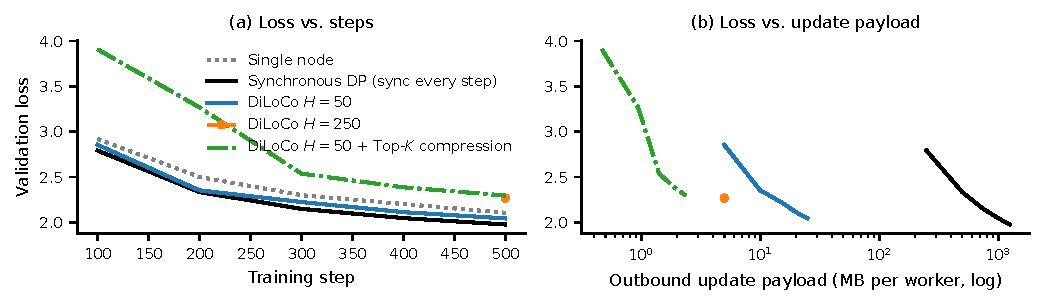
\includegraphics[width=\textwidth]{figures/eval_convergence.pdf}
\caption{Convergence--payload trade-off (0.62M parameters, TinyShakespeare, 3 workers, 500 steps). (a)~Validation loss by step. (b)~Loss versus cumulative outbound update payload estimate per worker: $50\times$--$250\times$ lower without compression and $527\times$ with compression.}
\label{fig:convergence}
\end{figure*}

\section{Robust Aggregation and Its Scope}
\label{sec:byzantine}

The experiments use equal-weight coordinate-wise Trimmed Mean and Median~\cite{yin2018byzantine}, and Multi-Krum~\cite{blanchard2017machine}. For Trimmed Mean,
\begin{equation}
 \bar g_j=\frac{\sum_{i\in\mathcal S_j}g_{i,j}}
 {N-2\lfloor\beta N\rfloor},
\end{equation}
where $\mathcal S_j$ removes each coordinate's extreme $\lfloor\beta N\rfloor$ entries at each end. A trim/breakdown fraction is not an unconditional convergence or backdoor guarantee. Unequal local trajectories, non-i.i.d. data, compression, and stage contamination need separate evaluation.

The earlier $\sqrt{B_i}$ work-weight policy is not Sybil resistant: splitting $B$ batches among $k$ identities yields total nominal influence $\sqrt{kB}$. Additional stakes impose a cost but do not erase that advantage. The target therefore separates task rewards from consensus power and contribution eligibility. The equal-weight experiments assume their worker population; they do not validate permissionless admission or a weighted robust estimator.

\subsection{Conditional Composition}

An elementary bound clarifies the verification target. Assume a valid genesis state, binding task/dependency commitments, deterministic transitions including aggregation, and no canonical use before the acceptance rule completes. Let $\epsilon_j$ bound the probability that check $j$ accepts an invalid transition conditional on a valid preceding history, and let $\delta_c$ bound a consensus safety failure. Induction over dependencies and a union bound give
\begin{equation}
 \Pr[\text{conflicting or invalid canonical history}]
 \leq \delta_c+\sum_{j=1}^{K}\epsilon_j
\end{equation}
over $K$ checks. No independence is required. Unavailable evidence must postpone acceptance rather than bypass verification. Establishing small $\epsilon_j$ against adaptive adversaries is an obligation, not a consequence of signatures or nominal sampling rates. Full deterministic replay with an honest executor and sound adjudication supplies a reference case.

Correct execution still does not prove optimization quality. For an $L_F$-smooth objective $F$ and a simpler reference step $\theta^+=\theta-\eta(\nabla F(\theta)+e)$, $0<\eta\leq1/L_F$, the smoothness inequality gives
\begin{equation}
 F(\theta^+)\leq F(\theta)-\tfrac{\eta}{2}\|\nabla F(\theta)\|^2
                   +\tfrac{\eta}{2}\|e\|^2.
\end{equation}
This follows by expanding the squared update norm; it is a sufficient descent condition, not a new convergence theorem. Verification constrains execution deviations, while data, stochasticity, local drift, and compression determine the remaining error. Extending this argument to the evaluated local AdamW/Nesterov hierarchy requires additional analysis.

\section{Evaluation}
\label{sec:eval}

Component experiments use NeuroLLM, its outer optimizer, compressor, robust aggregator, proof structures, and ECDSA primitives in in-process harnesses on a 4-vCPU host. Models are byte-level LMs on TinyShakespeare; raw results and harnesses are public. A separate native-chain reference tests computation-to-reward settlement under a narrower execution profile.



\subsection{Convergence versus Payload}

Three workers with disjoint shards train for 500 steps under synchronous data parallelism, DiLoCo with $H\in\{50,250\}$, and compressed DiLoCo $H=50$. Accounting for full parameter payloads, the synchronous baseline is 1.25\,GB/worker; $H=50$ is 25\,MB ($50\times$ lower) and ends 3.4\% above synchronous validation loss (2.04 vs.\ 1.98). $H=250$ trades 15\% final loss for $250\times$ lower payload; compression reaches $527\times$ (2.4\,MB) with $+16.2\%$ loss at step 500 (2.296 vs.\ 1.976). These counters exclude return traffic, pipeline tensors, checkpoints, audits, protocol framing, retries, and gossip duplication; they are not measured WAN traffic.

\subsection{Byzantine Robustness}
\label{sec:eval-byz}

\begin{figure}[t]
\centering
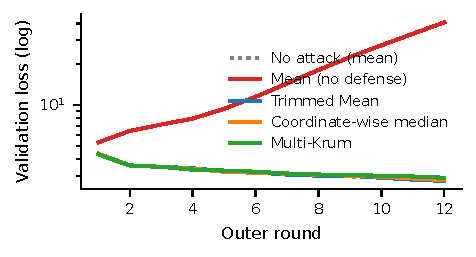
\includegraphics[width=\columnwidth]{figures/eval_byzantine.pdf}
\caption{Single-seed run: 10 workers, 3 adversarial, sign-flip attack, 12 rounds. Equal-weight robust estimators track the attack-free baseline.}
\label{fig:byzantine}
\end{figure}

\begin{table}[t]
\caption{Final validation loss after 12 outer rounds (10 workers, 30\% adversarial unless noted)}
\label{tab:byz}
\centering
\begin{tabular}{@{}lcc@{}}
\toprule
\textbf{Aggregation} & \textbf{Sign-flip} & \textbf{Noise} \\
\midrule
No attack (mean) & \multicolumn{2}{c}{2.83} \\
\midrule
Mean (no defense) & 40.67 & 2.52 \\
Trimmed Mean ($\beta{=}0.3$)~\cite{yin2018byzantine} & 2.75 & 2.82 \\
Coordinate-wise Median~\cite{yin2018byzantine} & 2.79 & 2.84 \\
Multi-Krum~\cite{blanchard2017machine} & 2.90 & 2.90 \\
\midrule
Trimmed Mean, $f{=}10\%$ / $20\%$ & 2.87 / 2.84 & --- \\
Trimmed Mean, $f{=}40\%$ (above trim) & 19.04 & --- \\
\bottomrule
\end{tabular}
\end{table}

Three of 10 workers submit either sign-flipped updates ($\Delta w\mapsto-5\Delta w$) or zero-mean Gaussian noise at $10\times$ honest magnitude. Under sign-flip, mean aggregation diverges (40.7 vs.\ 2.83), whereas the three robust estimators finish at 2.75--2.90 (Table~\ref{tab:byz}, Fig.~\ref{fig:byzantine}). For Trimmed Mean, 10/20/30\% remain near baseline (2.87/2.84/2.75), while 40\% degrades sharply (19.0). In this single-seed, small-model experiment, the result describes complete worker updates under the specified attacks; it does not establish the pipeline or admission assumptions in Section~\ref{sec:design}.

\subsection{Compression, PoNW Overheads, and Churn}
\label{sec:eval-comp}

\textbf{Compression.} On 50-step pseudo-gradients, Top-$K=5/10/20\%$ with int8 and zlib yields $20.6\times/10.8\times/5.6\times$ reduction at cosine fidelity 0.46/0.58/0.73; error feedback recycles discarded mass.
\textbf{PoNW.} A serialized cohort-sync proof is 763 bytes; ECDSA signing and verification take 1.5\,ms and 0.56\,ms. A standalone forward/backward batch takes ${\sim}97$\,ms, illustrating one replay unit but \emph{not} measuring full challenge resolution.
\textbf{Churn.} In a three-node Docker LAN, killing one node at $t=123$\,s leaves survivors advancing ($642\to2070$ aggregate steps). In a 10-minute kill/restart run, the node rejoins via tracker/DHT, performs 583 further steps, and continues descending (loss 0.19 vs.\ 0.04 for uninterrupted peers). A 15-minute run sustains 4{,}721 steps without crashes. The restart report uses full replicas holding layers [0,1]; these local losses and step counters do not validate partitioned-model recovery or canonical checkpoint agreement.

\subsection{Native-Chain Reference Demonstrator}

On one 4-vCPU host, four CometBFT 0.38.26 validators run a separate NeuroShard genesis, each with a durable Python application. Two worker processes hold disjoint stages of a 34,976-parameter NeuroLLM. They execute real forward/backward tasks; all validators independently replay each complete SGD step and check signed gradient/boundary commitments. Genesis fixes the numerical profile, corpus digest, program hash, and development issuance cap.

Fifteen accepted steps reduce a fixed held-out batch loss from 5.741 to 4.110. Settlement issues exactly 15 development NEURO, split equally between workers. Incorrect results, signed incorrect gradients, and repeated claims earn no reward. Three surviving validators finalize training; two cannot finalize a queued valid transaction during a four-second observation. After restart, all four agree on the model, balances, a common block hash, and inference output. Twenty unit tests also check exact stage/full-model gradients and durable replay after an interrupted commit. The reproduction command is \texttt{python scripts/demo\_neuroshard.py check}. These results test local composition with fixed validators, full replay, and one CPU profile; they do not establish permissionless security or useful inference quality.

\section{Limitations and Research Priorities}

The reference implements native consensus integration, stage/full-model replay, and atomic training rewards. Public validator admission, availability enforcement, paid verification, and dispute economics remain proposed. Evidence is small-scale: fixed local validators do not provide decentralized ownership, and full replay requires every validator to hold the model. Robust estimation, correct execution, consensus agreement, and useful learning remain distinct guarantees.

The next gates are independent-machine reproducibility and adversarial consensus tests; open resource-based admission and reconfiguration; available-state disputes and collateral accounting; and multiple-seed attacks under complete WAN cost accounting. Runtime diversity, genesis distribution, audit incentives, and data governance require explicit evaluation before a public network.

NeuroShard's opportunity is to make independent model shards contribute to an auditable shared computation. The reference gives accepted tasks, payments, and checkpoints one reproducible protocol meaning; scaling that property to an open network is the next research obligation.

\bibliographystyle{IEEEtran}
\begin{thebibliography}{00}
\bibitem{douillard2023diloco}
A.~Douillard \emph{et~al.}, ``DiLoCo: Distributed low-communication training of language models,'' \emph{arXiv:2311.08105 [cs.LG]}, Nov. 2023.

\bibitem{jaghouar2024opendiloco}
S.~Jaghouar, J.~M.~Ong, and J.~Hagemann, ``OpenDiLoCo: An open-source framework for globally distributed low-communication training,'' \emph{arXiv:2407.07852 [cs.LG]}, Jul. 2024.

\bibitem{jaghouar2024intellect}
S.~Jaghouar \emph{et~al.}, ``INTELLECT-1 technical report,'' \emph{arXiv:2412.01152 [cs.DC]}, Dec. 2024.

\bibitem{ryabinin2023swarm}
M.~Ryabinin, T.~Dettmers, M.~Diskin, and A.~Borzunov, ``SWARM parallelism: Training large models can be surprisingly communication-efficient,'' in \emph{Proc.\ ICML}, vol.~202, 2023, pp.~29416--29440.

\bibitem{sani2024photon}
L.~Sani \emph{et~al.}, ``Photon: Federated LLM pre-training,'' \emph{arXiv:2411.02908 [cs.LG]}, Nov. 2024.

\bibitem{borzunov2023petals}
A.~Borzunov \emph{et~al.}, ``Petals: Collaborative inference and fine-tuning of large models,'' in \emph{Proc.\ ACL: System Demonstrations}, 2023, pp.~38--44.

\bibitem{lidin2025gauntlet}
J.~Lidin, A.~Sarfi, E.~Pappas, S.~Dare, E.~Belilovsky, and J.~Steeves, ``Incentivizing permissionless distributed learning of LLMs,'' \emph{arXiv:2505.21684}, 2025.

\bibitem{lidin2026covenant}
J.~Lidin \emph{et~al.}, ``Covenant-72B: Pre-training a 72B LLM with trustless peers over-the-internet,'' \emph{arXiv:2603.08163}, 2026.

\bibitem{avraham2026agora}
G.~Avraham \emph{et~al.}, ``Agora: Collective and permissionless internet-scale pretraining of large language models,'' \emph{arXiv:2607.13332}, 2026.

\bibitem{jia2021proof}
H.~Jia \emph{et~al.}, ``Proof-of-learning: Definitions and practice,'' in \emph{Proc.\ IEEE S\&P}, 2021, pp.~1039--1056.

\bibitem{zhang2022adversarial}
R.~Zhang \emph{et~al.}, ```Adversarial examples' for proof-of-learning,'' in \emph{Proc.\ IEEE S\&P}, 2022, pp.~1408--1422.

\bibitem{fang2023proof}
C.~Fang \emph{et~al.}, ``Proof-of-learning is currently more broken than you think,'' in \emph{Proc.\ IEEE EuroS\&P}, 2023, pp.~797--816.

\bibitem{ong2025toploc}
J.~M.~Ong \emph{et~al.}, ``TOPLOC: A locality sensitive hashing scheme for trustless verifiable inference,'' \emph{arXiv:2501.16007 [cs.CR]}, Jan. 2025.

\bibitem{arun2025verde}
A.~Arun \emph{et~al.}, ``Verde: Verification via refereed delegation for machine learning programs,'' \emph{arXiv:2502.19405}, 2025.

\bibitem{yin2018byzantine}
D.~Yin, Y.~Chen, K.~Ramchandran, and P.~Bartlett, ``Byzantine-robust distributed learning: Towards optimal statistical rates,'' in \emph{Proc.\ ICML}, vol.~80, 2018, pp.~5650--5659.

\bibitem{blanchard2017machine}
P.~Blanchard, E.~M.~El~Mhamdi, R.~Guerraoui, and J.~Stainer, ``Machine learning with adversaries: Byzantine tolerant gradient descent,'' in \emph{Adv.\ NeurIPS}, vol.~30, 2017, pp.~118--128.

\bibitem{baruch2019little}
M.~Baruch, G.~Baruch, and Y.~Goldberg, ``A little is enough: Circumventing defenses for distributed learning,'' in \emph{Adv.\ NeurIPS}, vol.~32, 2019.

\bibitem{buchman2019tendermint}
E.~Buchman, J.~Kwon, and Z.~Milosevic, ``The latest gossip on BFT consensus,'' \emph{arXiv:1807.04938}, 2019.

\bibitem{douceur2002sybil}
J.~R.~Douceur, ``The Sybil attack,'' in \emph{Proc.\ IPTPS}, 2002, pp.~251--260.

\end{thebibliography}
\end{document}
